\documentclass[main.tex]{subfiles}
\begin{document}

由于各部分说明中此部分重复给出各个Project的系统总体框图,便于观察和对比。

\begin{figure}[h]
  \begin{adjustbox}{addcode={\begin{minipage}{\width}}{\caption{Project1 顶层模块mips框图}\end{minipage}},rotate=90,center}
		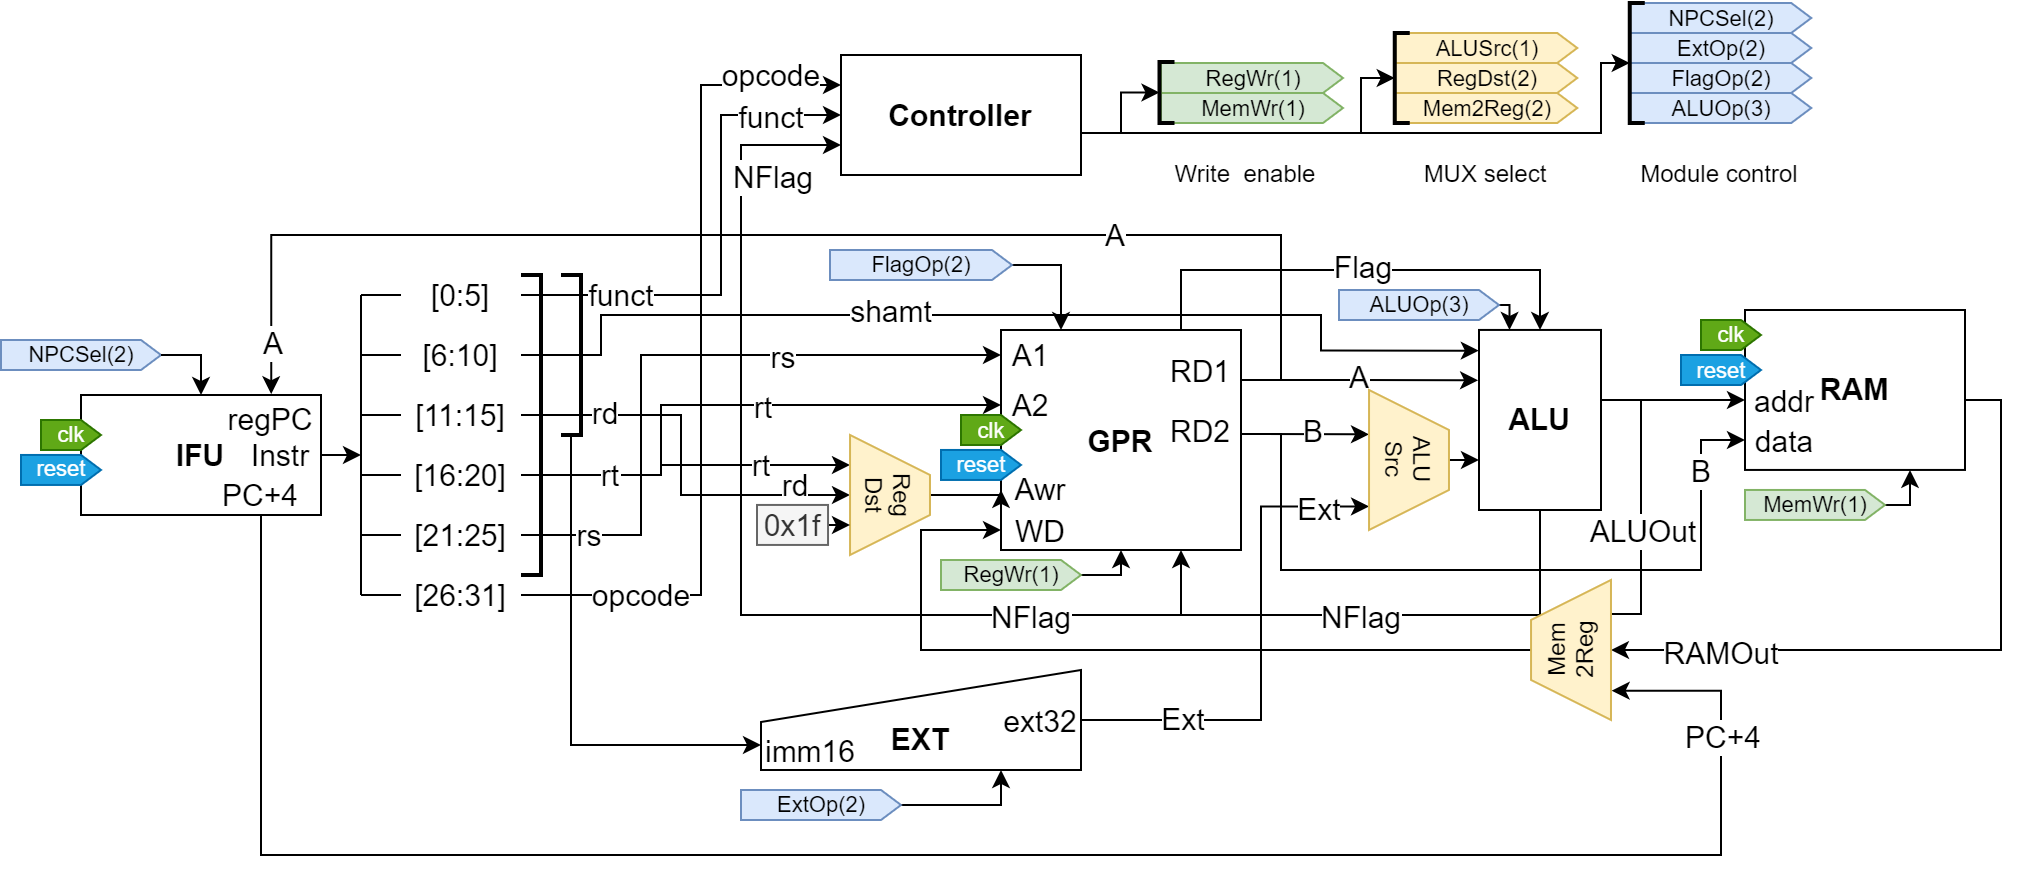
\includegraphics[width=10 in]{images/PCOCD-P1-overall-block.png}%
	\end{adjustbox}
\end{figure}
\clearpage

\begin{figure}[h]
  \begin{adjustbox}{addcode={\begin{minipage}{\width}}{\caption{Project2 顶层模块mips框图}\end{minipage}},rotate=90,center}
		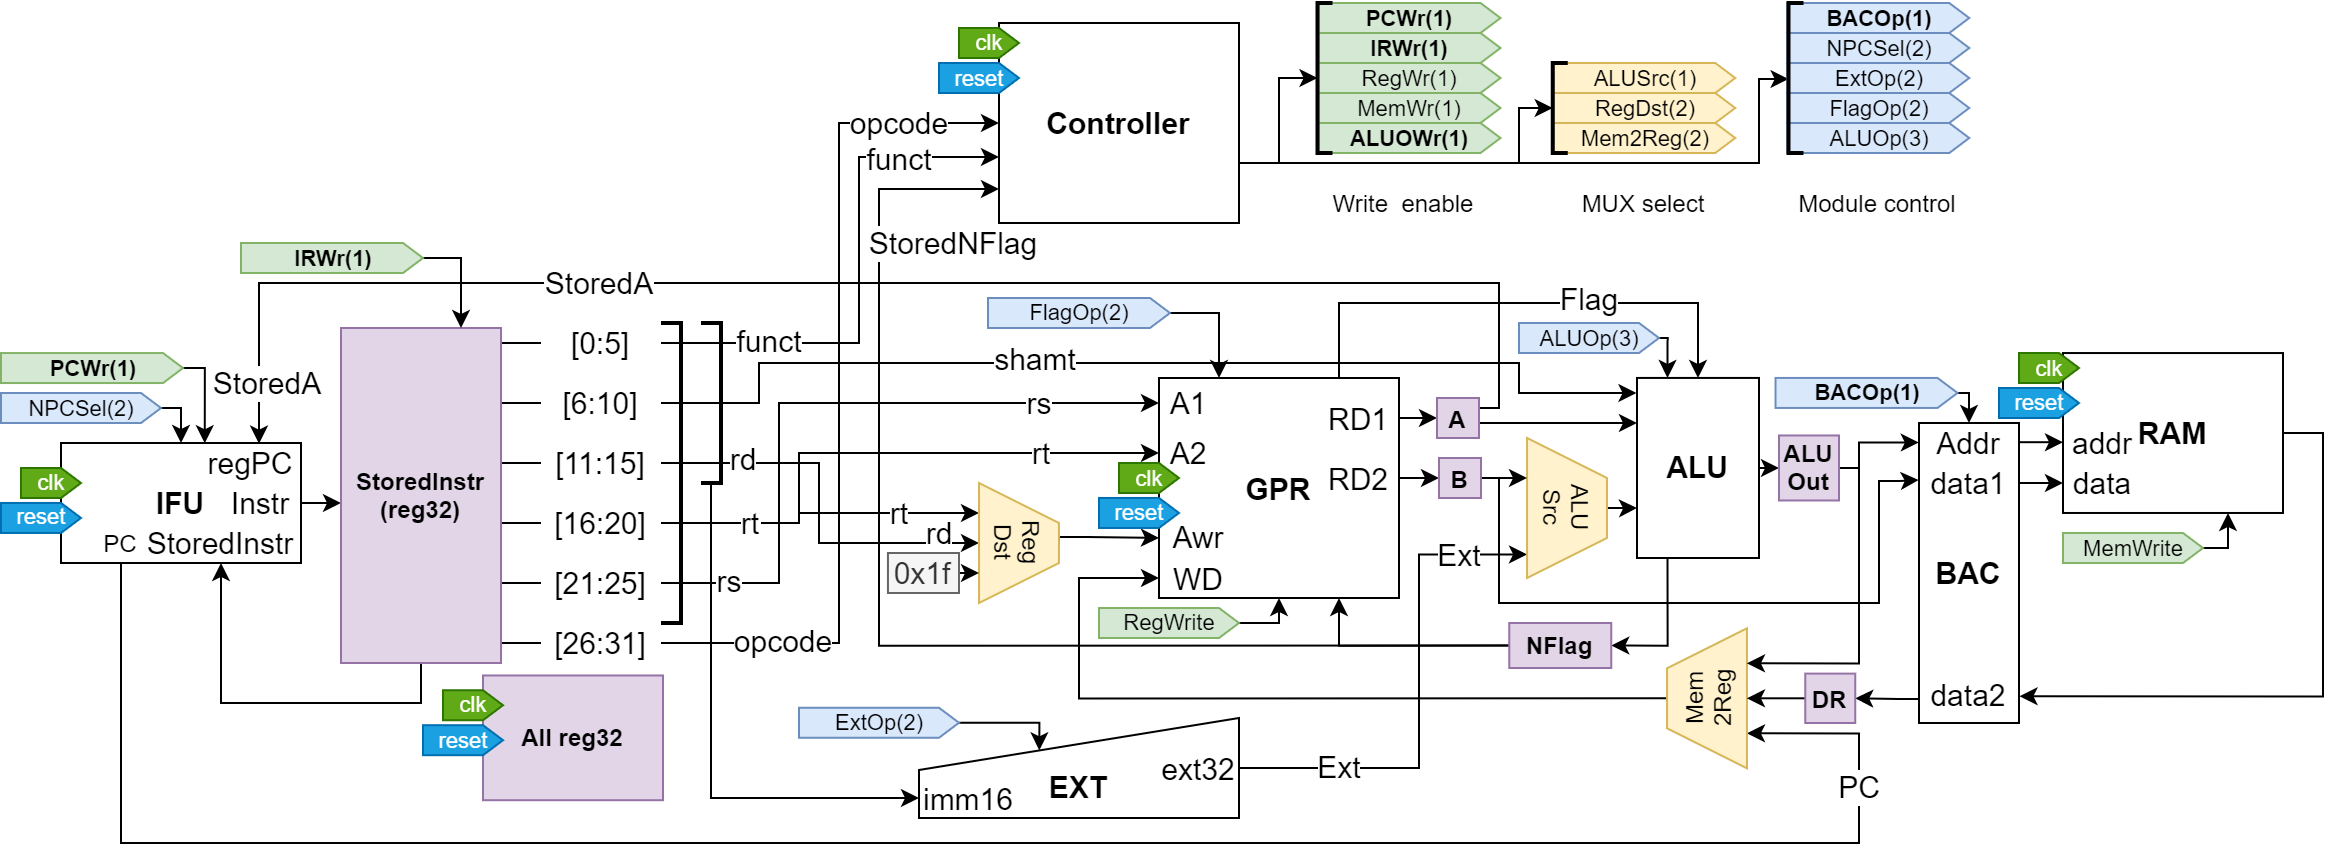
\includegraphics[width=10 in]{images/PCOCD-P2-overall-block.png}%
	\end{adjustbox}
\end{figure}
\clearpage

\begin{figure}[h]
  \begin{adjustbox}{addcode={\begin{minipage}{\width}}{\caption{Project3 CPU模块mips框图}\end{minipage}},rotate=90,center}
		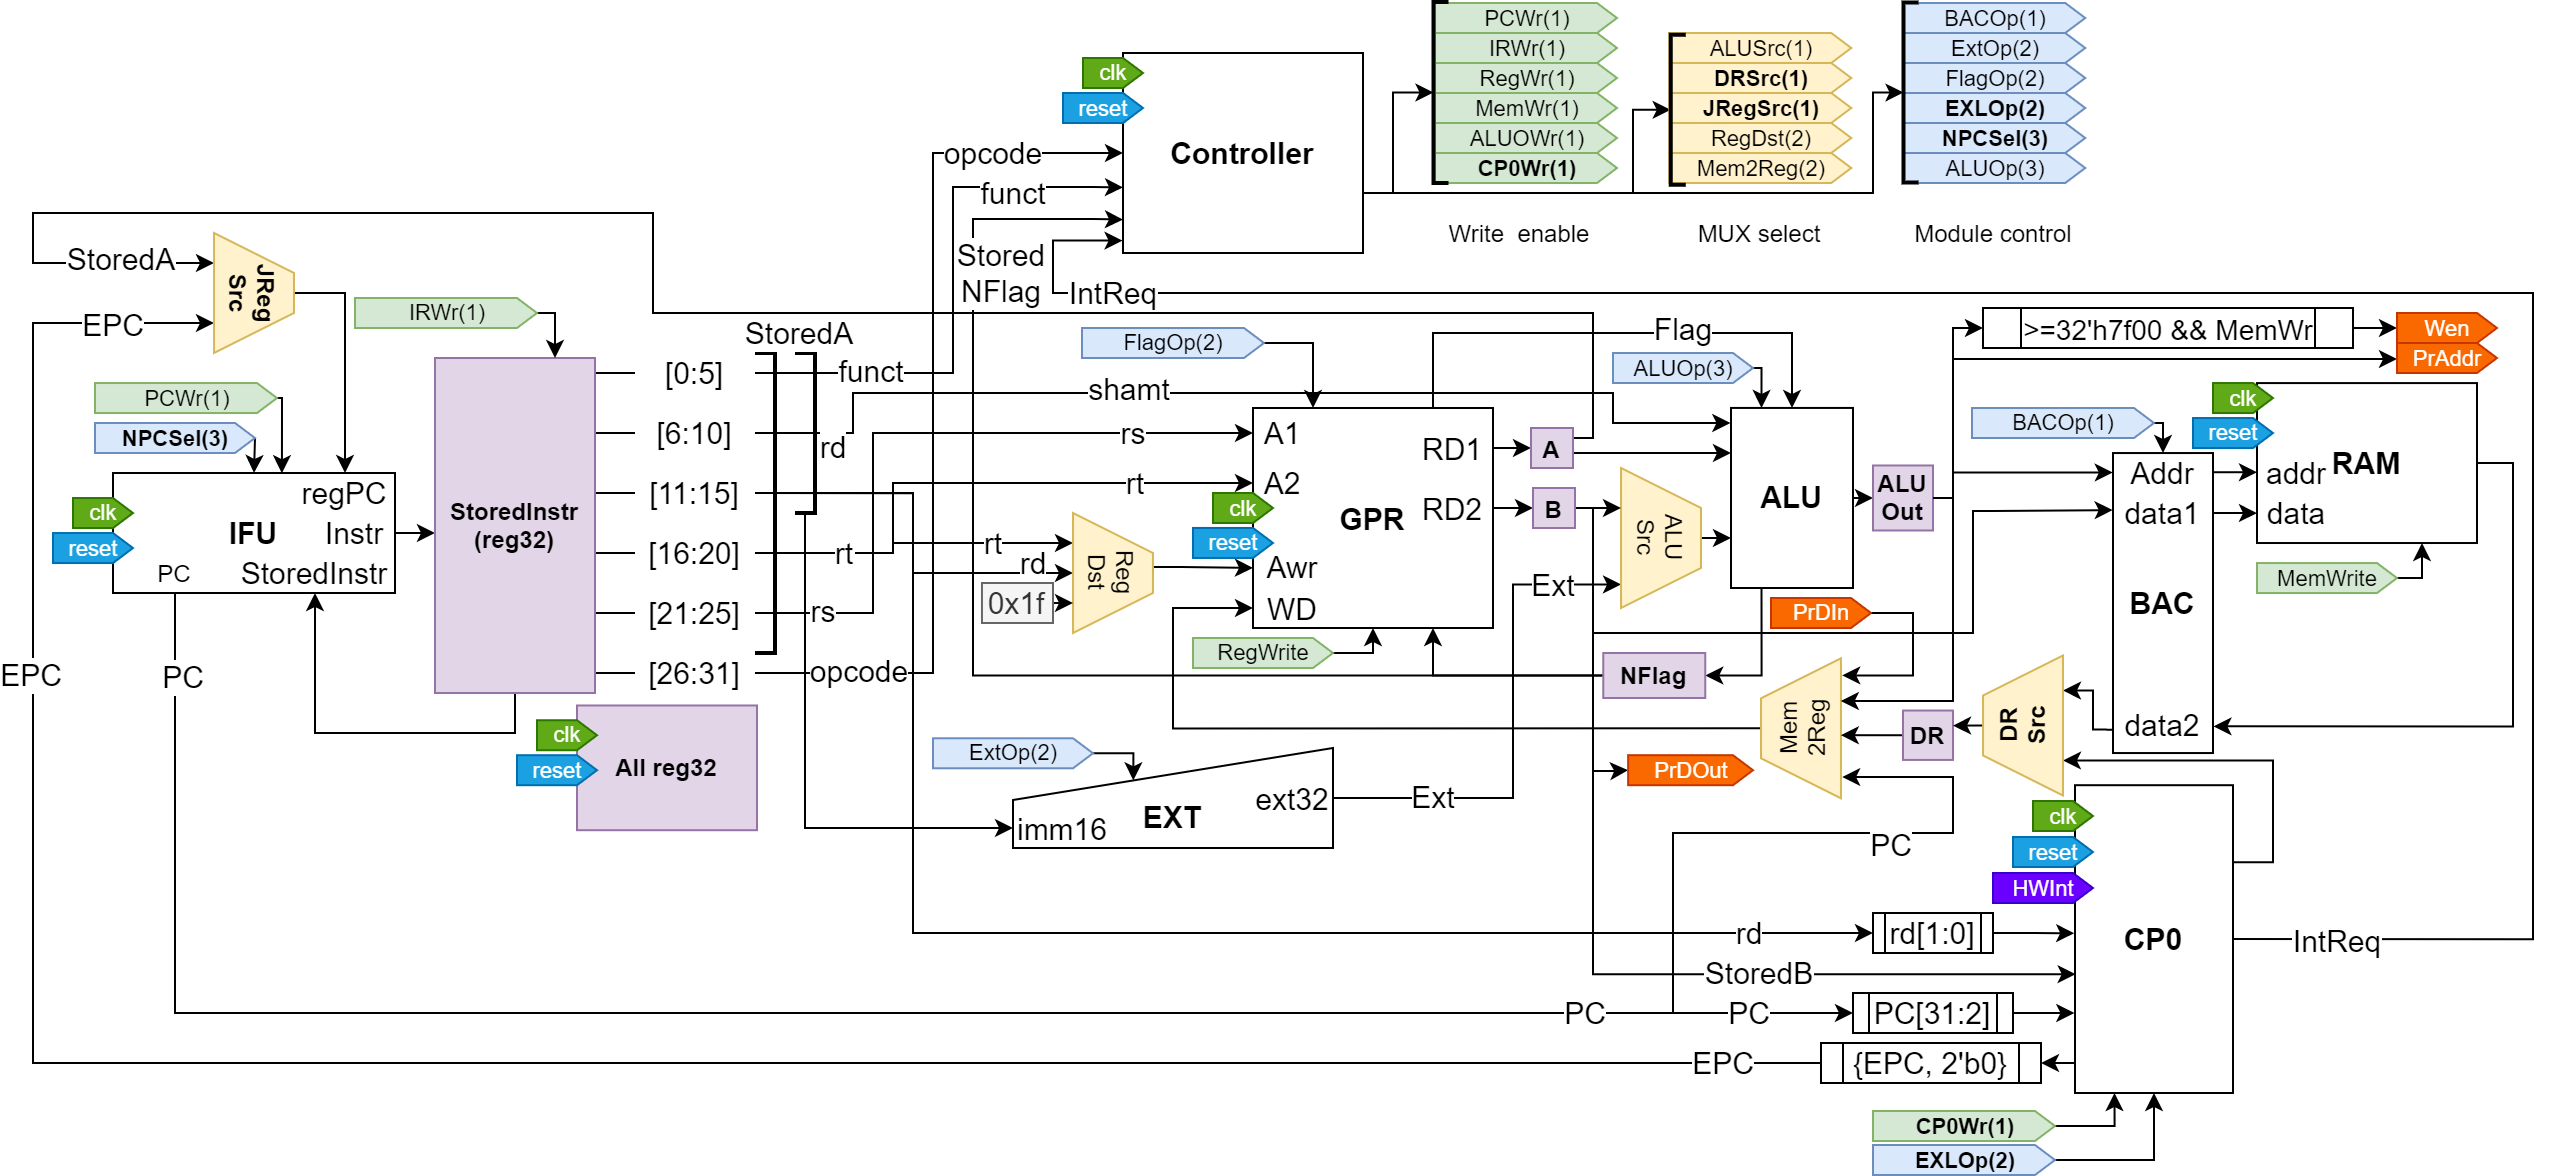
\includegraphics[width=10 in]{images/PCOCD-P3-mips-block.png}%
	\end{adjustbox}
\end{figure}
\clearpage

\begin{figure}[h]
  \begin{adjustbox}{addcode={\begin{minipage}{\width}}{\caption{Project3 顶层模块main框图}\end{minipage}},rotate=90,center}
		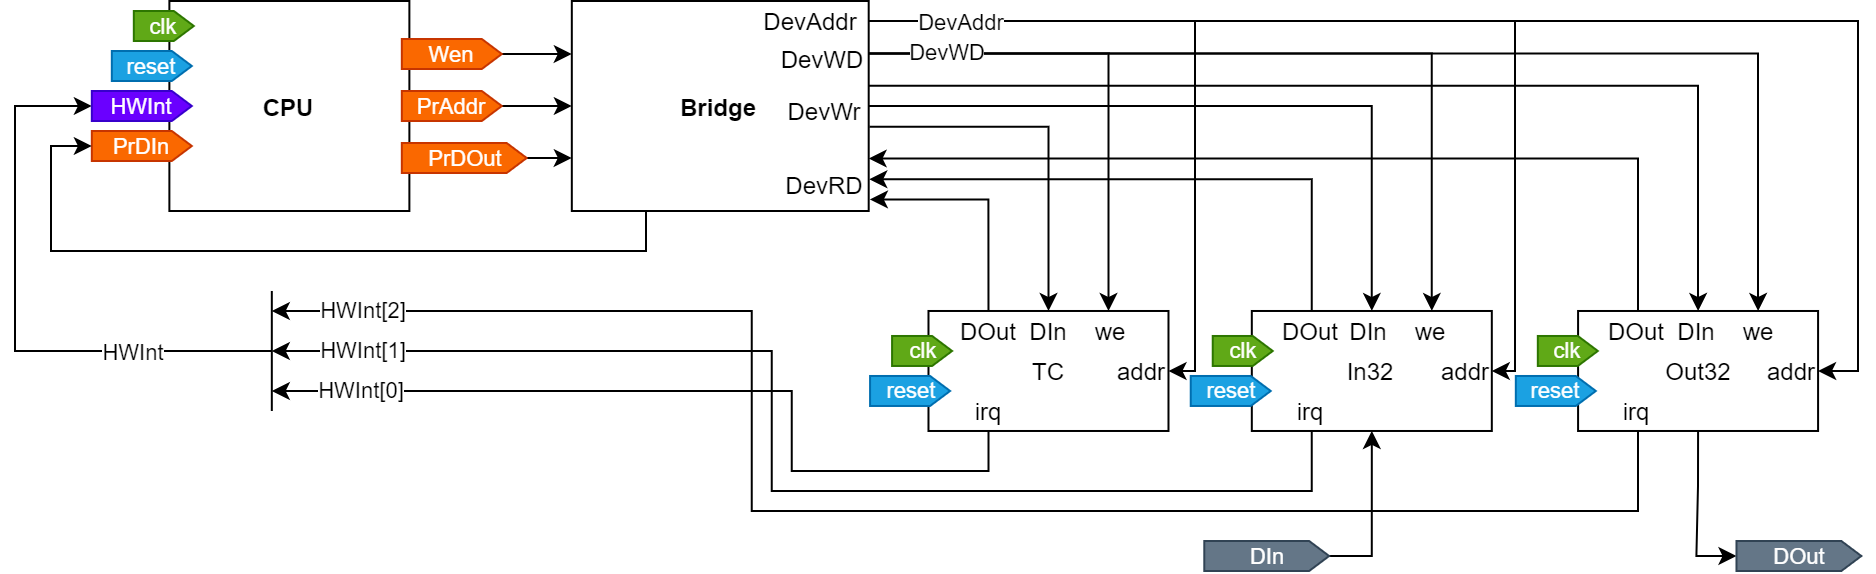
\includegraphics[width=10 in]{images/PCOCD-P3-main-block.png}%
	\end{adjustbox}
\end{figure}
\clearpage

\begin{figure}[h]
  \begin{adjustbox}{addcode={\begin{minipage}{\width}}{\caption{Project4 顶层模块pratical框图}\end{minipage}},rotate=90,center}
		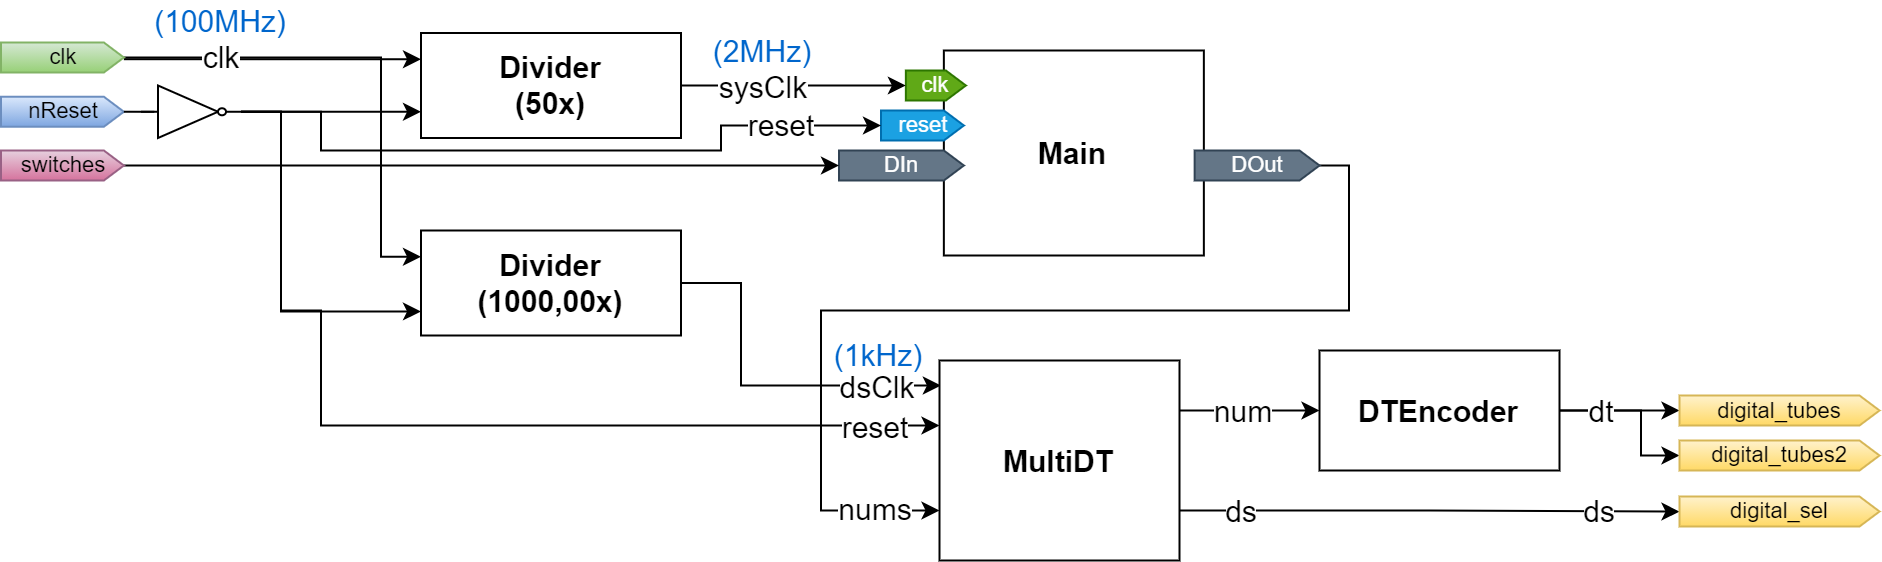
\includegraphics[width=10 in]{images/PCOCD-P4-pratical-block.png}%
	\end{adjustbox}
\end{figure}
\clearpage

\end{document}